% THIS IS SIGPROC-SP.TEX - VERSION 3.1
% WORKS WITH V3.2SP OF ACM_PROC_ARTICLE-SP.CLS
% APRIL 2009
%
% It is an example file showing how to use the 'acm_proc_article-sp.cls' V3.2SP
% LaTeX2e document class file for Conference Proceedings submissions.
% ----------------------------------------------------------------------------------------------------------------
% This .tex file (and associated .cls V3.2SP) *DOES NOT* produce:
%       1) The Permission Statement
%       2) The Conference (location) Info information
%       3) The Copyright Line with ACM data
%       4) Page numbering
% ---------------------------------------------------------------------------------------------------------------
% It is an example which *does* use the .bib file (from which the .bbl file
% is produced).
% REMEMBER HOWEVER: After having produced the .bbl file,
% and prior to final submission,
% you need to 'insert'  your .bbl file into your source .tex file so as to provide
% ONE 'self-contained' source file.
%
% Questions regarding SIGS should be sent to
% Adrienne Griscti ---> griscti@acm.org
%
% Questions/suggestions regarding the guidelines, .tex and .cls files, etc. to
% Gerald Murray ---> murray@hq.acm.org
%
% For tracking purposes - this is V3.1SP - APRIL 2009

\documentclass{acm_proc_article-sp}

\begin{document}



\title{Catchy Part: Surveying Users' Perceptions of Threats for Wearable Devices}
%\titlenote{(Does NOT produce the permission block, copyright information nor page numbering). For use with ACM\_PROC\_ARTICLE-SP.CLS. Supported by ACM.}}

%\subtitle{[Extended Abstract]
%\titlenote{Note
%\textit{Note \LaTeX$2_\epsilon$\ and BibTeX} at \texttt{www.website.com}}}


\numberofauthors{3} 

\author{
% 1st. author
\alignauthor
Linda N. Lee\\
       \affaddr{UC Berkeley}\\
       \email{lnl@cs.berkeley.edu}
% 2nd. author
\alignauthor
Serge Egelman\\
       \affaddr{UC Berkeley}\\
       \affaddr{ICSI}\\
       \email{serge@cs.berkeley.edu}
% 3rd. author
\alignauthor David Wagner\\
       \affaddr{UC Berkeley}\\
       \email{daw@cs.berkeley.edu}
}

\maketitle



\begin{abstract}
(Okay, kind of intimidated with writing the abstract. My plan is to write intro/conclusion first and then condense it into here, while nodding off to the contributions that we made.) At the very least, I can say that we studied user perceptions for threats in wearable devices, along with user perceptions of risk and benefit for emerging technologies and what they thought was the biggest risk for using wearable devices. Data type, data recipient, and device type all matter different amounts. All new technologies were perceived to be low risk low benefit but we think this is because people are unfamiliar with these technologies. Privacy was the number one concern, followed by security, then health, money, social norms changing and social stigma. Fantastic ending sentence here.
\end{abstract}

% A category with the (minimum) three required fields
\category{look it up}{keyword1}{keyword2}{keyword3}
%A category including the fourth, optional field follows...
%\category{D.2.8}{Software Engineering}{Metrics}[complexity measures, performance measures]

\terms{term1} {term2} {term3}

\keywords{Privacy, Security, User Studies, Risk Perception, Ubiquitous Computing, Wearables} % NOT required for Proceedings

%%%%%%%%%%%%%%%%%%%
%%%         PAPER BODY         %%%
%%%%%%%%%%%%%%%%%%%


%%%%% FEEDBACK TO INCORPORATE, from Serge

%-"security and privacy concerns regarding wearable devices are becoming heightened as companies make headlines for incidents resulting in users’ sexual activities exposed to the public..." I would rewrite this. You don't really mean to say that tracking sexual activity is the *only* privacy and security concern. It's one of many. I would say at the beginning that there are myriad privacy/security concerns, and then go into specific examples (e.g., sex, facial recognition, etc.).
%-I think you might want to motivate this better: why do we need to better understand the threat landscape? (Answer: to focus on the most concerning things and then warn users when they're about to occur or prevent them from happening altogether.)
%-Start a new paragraph before the contribution bullets to say what we actually did. For example, "we surveyed 2,250 Internet users to determine..."
%-For the bullets, these can be made much more concise. I would also frame them in terms of what we found, not what we did. For example, "we found that X% of participants found that Y threats were most concerning..."
%-I would limit these bullets to the top 3-4 most interesting findings that we found.

\section{Introduction}
Wearable technology has many potential benefits, ranging from a more natural, human-centered interface for computing to healthier living through fitness tracking. Wearable devices, or ``wearables,'' are the new frontier of ubiquitous computing and big data, constantly capturing data and interpreting information to deliver insights to the user. Wearbles are gaining lots of attention. Forbes has named 2014 the ``Year of Wearable Technology \cite{Forbes},'' and market research companies estimate that 52\% are aware of wearables and among those, 33\% said they were likely to buy one \cite{NPD}. 

A survey consisting of 3,956 respondents who are either current users or non-users with high interest in wearables found that most popular devices are fitness bands (61\%), followed by smart watches (45\%) and mobile health devices (17\%)\cite{Nilsen}. It is estimated that 20\% of the general population own at least one wearable and 10\% use at least one wearable in their daily lives \cite{WearableStatNews}. The demographics of wearables consumers are young and affluent--48\% of owners are between 18 and 34 years old, and 29\% make over \$100,000 per year. However, it is expected that this \$700 million industry will reach other demographics soon as the prices of wearable devices drop \cite{cmo}. 

Even in early adoption, security and privacy concerns regarding wearable devices are becoming heightened. Many of these concerns relate to users' activities being exposed to the public without awareness or consent. For instance, Fitbit's fitness profiles were public by default and also allowed users to track sex as an exercise\cite{Fitbit}, resulting in disclosing sensitive information about the user. In other instances, public discomfort prevented certain capabilities from being enabled. Google's Glass had to disable facial recognition for Glass upon release \cite{GlassDetection}. 

To avoid both scandalous breaches of privacy and public opposition to new capabilities, it is critical that we understand the threat landscape for wearable devices and which issues users most care about--before wearbles become increasingly more ubiquitous and powerful \cite{Implants}. A better understanding of the threat landscape will enable researchers and companies alike to focus on the most concerning factors for the user--allowing research for effective warnings of relevant events and an informed focus of protecting the data of high priority.

We surveyed 2,250 internet users to determine what data is sensitive, which technologies are risky, and what users think are the biggest risk for operating wearable devices. In this work, we contribute the following: \\[-0.8cm]

\begin{itemize} \itemsep1pt \parskip0pt \parsep0pt
\item We show users' perceptions of a wide range of wearables threats, along with an evaluation of which factors contribute to the severity of a threat. We find that data type and data recipient matter, but the device type does not.  
\item We investigate how people's privacy preferences differ when data is perceived to be shared with people or a server.
\item We show risk and benefit assessments of new technologies and capabilities relative to better understood technologies.  Most are perceived as low-risk/low-benefit, but we hypothesize this is  the result of limited exposure. 
\item We report people's self-reported top concerns for wearable devices. Privacy, by far, is the top concern. Other notable risks include information security, long-term health risks from use, high financial cost, and change in social norms. 
\end{itemize}

%%%%%%%%%%%%%%%%%%%

\section{Related Work}
In this section, we discuss related work which explores threats for smartphones and wearable devices, discusses emerging challenges related to ubiquitous computing, and studies user perceptions of threats and technologies. 

\subsection{Concerns for Smartphones and Wearables}
(REDO) Mention Adrienne's work here, and other relevant smartphone studies of any sort. I will talk about how I model Adrienne's work in the next section, Survey, just give a nod to it here and go into it later. Since my results were that people care about privacy, security, health, and social change/social stigma, any phone studies which hint at any of those things will be good to put here. Be sure to go cite a fair number of them. Related work section is the part where it looks like I know stuff. 

Mention any studies for wearables (like the ones you can find at Ubicomp, CHI, or SOUPS), and give them a nod. Especially mention ones on privacy and perceptions, since I know those exist. I doubt there will be ones for social norm shifts/social stigma, or health concerns, but maybe I can at least include some security ones here too. Throughout mentioning all of these works, highlight how my study is different from previous studies. 

\subsection{Ubiquitous Computing}
(REDO) As technology becomes more and more ubiquitous, more sensors will record more things about more people more of the time. There are an endless amount of unique situations which can negatively impact a person's privacy or security. There is a clear need to better communicate these risks to people (cite webcam paper and other papers here?), but there are too many things to warn people about. Therefore, we need to know what are the most threatening and also most relevant situations to inform the users about, since we can't bug them all the time about everything. 

We need to investigate the threat landscape and people's privacy concerns now, before wearables are widely adopted, or designed without these considerations in mind. So although our research is at at time when things are rapidly changing and most people don't have wearables, it is crucial to do the research now so we can prevent badness later.

\subsection{User Perception}
(REDO) In this paper, we investigate one of the two important questions--what are the most relevant situations to people. We do this firstly because people are really bad at knowing the likelihood of something, especially a threat with respect to security or privacy, is going to happen (sources here). And while the most damaging situations should also be addressed, this is not yet possible since these technologies haven't been adopted and the damage hasn't happened, so we don't know yet. Additionally, since the number one concern that people had with these devices was privacy (can I say result here? I guess I already did in abstract), we need to know what people consider private, which is more nuanced and requires a user study like this survey. 

We also study risk. Mention Fischoff here. This is a very seminal paper in risk perception and it also studies how safe enough something has to be before people can accept something. I will talk about how I model my work in the next section, Survey, just give it a nod here and go into it later. Also mention at least a couple more works related to risk perception here to round it off. 

%%%%%%%%%%%%%%%%%%%

\section{Methodology}
Our survey was conducted in multiple parts. The first section of the survey consisted of questions regarding individual and situational concerns with respect to a fictitious wearable device called the Cubetastic3000 (done to prevent biases in answers from participants with respect to specific artifacts or companies). The next section of questions consisted of questions regarding individual and situational smartphone concerns, which were questions more familiar to our participant base and are used for calibrating results. The following section of the survey consisted of risk and benefit assessment of technologies, where participants were asked to consider general, multi-situational concerns regarding specific technologies. The final section of the survey consisted of demographics questions on basic information, privacy concerns, and wearable device ownership. Details on the question ordering, question formatting, and sample questions are discussed in the remainder of this section. 

%%% commented out for anonymity; can comment back in later.
%The full survey can be found at http://www.surveygizmo.com/s3/1657924 /Wearables-Threats-User-Survey. 

%In total, the survey consisted of 367 unique questions, with each participant answering 27 questions. Out of the 27 seen by each participant, 17 of the questions were constant, whereas 10 of the questions were selected at random from larger sets of questions.

During the course of the survey, each participant answered 27 questions:   \\[-.8cm]

\begin{itemize} \itemsep1pt \parskip0pt \parsep0pt
\item 2 comprehension questions (attention checks)
\item 6 questions about various wearables scenarios 
\item 2 questions about smartphone scenarios 
\item 2 risk/benefit questions 
\item 15 demographics questions \\[-.8cm]
\end{itemize}

To mitigate any biases, the order in which question groups appeared to the user, the ordering within each group, and, when applicable, the order of the answers for questions, were randomized for each user. Details with respect to the relevant section of the survey are discussed in the respective subsections below.  

\subsection{Question Format} 
We talk about the format and justification of the questions from our survey below.

\subsubsection{Comprehension Questions}
Because we were asking questions about a fictitious device, participants were presented with two comprehension questions before the start of the wearable device scenarios questions. These questions served to ensure that participants would be informed of the device which we were going to be referring to, but also served as a filter for people who were inattentive or chose not to answer questions correctly. Filtering incomplete and incorrect responses to either of these comprehension questions filtered out 16\% (n = 366) of our participants. 

\subsubsection{Wearables Scenarios}
%okay, this section is kind of confusing, I must admit..  

After participants answered the two comprehension questions, participants were presented with 6 randomly selected questions from a set of 304 questions on various scenarios which can occur when wearing the Cubetastic3000. Out of these 304 questions, 292 (73 <data> * 4 <recipient>) were questions of the format: \textit{``How would you feel if an app on your Cubetastic3000 learned <data> and shared it with <recipient>, without asking you first?''}. 

The main purposes of these questions were to, firstly, determine how much the device, data type, and data recipient played a role in determining if a person was upset by an event or not and, secondly, to investigate what information would most upset users when shared. Additionally, there were 13 questions which did not follow the above format, lacking <data> to be shared and/or a <recipient>.  The 13 exploratory questions were additional scenarios which did not fit the standard question format but were relevant to ask our participants. An example of a regular question, a calibration question, and exploratory question, respectively, are below:  

standard: \textit{How would you feel if an app on your Cubetastic3000 learned how you were feeling based on your heart rate and shared that with the public, without asking you first?}\\[-.5cm]

exploratory: \textit{How would you feel if an app on your Cubetastic3000 turned your device off, without asking you first?}\\[-.5cm]

\subsubsection{Smartphone Scenarios}
Following the wearables scenario questions were 2 randomly selected questions from a set of 5 questions on various scenarios which can occur when using a smartphone. Unlike the wearables scenario questions, these questions only ask about various situations which may occur using a smartphone, without a <data> or <recipient>. These five scenarios, ranging from the most upsetting scenario to the least upsetting scenario, were purposefully selected from Felt et. al's mobile user study \cite{Felt} for eliciting varying reactions from users. 

calibration: \textit{How would you feel if an app on your Cubetastic3000 connected to a Bluetooth device (like a headset) without asking you first?} \\[-.5cm]

These questions were the basis for the five calibration wearables scenarios from the above section. Because we asked users questions differing only by the device in question, we are able to see how the change in device changes users' risk perception. Additionally, we compare our participants' perceptions of wearable device scenarios with existing perceptions of mobile device scenarios. Of the 13 exploratory questions in the wearables section, 5 of those questions were to calibrate with existing privacy work for smartphones and the other 7  were exploratory questions. These wearables questions, like the smart phone questions, were modeled after the mobile user study conducted by Felt et. al \cite{Felt}, but we ask the same questions but with respect to wearables rather than smart phones, to see if a change in device changes users' risk perception.


\subsubsection{Risk and Benefit Assessment}

In addition to investigating personal reactions to particular scenarios, we also wanted to study broad perceptions of various new technologies.We asked participants to evaluate the of following 20 new technologies: internet, email, laptops, smartphones, smart watches, fitness trackers, Google Glass, Cubetastic3000, discrete camera, discrete microphone, facial recognition, facial detection, voice recognition, voice based emotion detection, location tracking, speech to text, language detection, heart rate detection, age detection, and gender detection. 

For risk and benefit assessment, a technology was randomly selected for each participant, then risk and benefit questions for the same technology were selected for the participant. Each participant saw 1 risk assessment question and 1 benefit assessment question, in a randomized order. These questions ask about four previously studied technologies from the the seminal risk perception study by Fischhoff \cite{Fischhoff} (handguns, motorcycles, lawnmowers, and electricity), and 1 of the 20 new technologies.  Participants were asked to rate the same randomized new technology for both risk and benefit assessment. The format of the questions were as follows:

\textit{Fill in your risk/benefit numbers for the following technologies:}\\[-.5cm]

\textit{Handguns}: \_\_\_\_\_\_\_ \\
\textit{Motorcycles}: \_\_\_\_\_\_\_\\
\textit{Lawnmowers}: \_\_\_\_\_\_\_\\
\textit{<Wearable Technology>}: \_\_\_\_\_\_\_\\
\textit{Electricity}: \_\_\_\_\_\_\_\\ [-.5cm]

To parallel the risk perception study, we gave our participants a similar prompt which instructed them to numerically express the conceived gross risk/gross benefit for a long period of time for all parties involved. The prompt can be seen in appendix \ref{sec:prompt}. 

\subsubsection{Additional Questions}
The exit portion of the survey consisted of demographics questions to better understand the answers. We included standard demographics questions such as age, gender, and education, but also asked participants if they owned a wearable device to survey the population's exposure to these devices. We also prompted them with an open-ended question on what would be the most likely risks associated with wearable devices, and finished with questions from a privacy index to gauge their privacy preferences. We used the Internet Users' Information Privacy Concerns (IUIPC) index \cite{malhotra2004internet}.

\subsection{Focus Group}
We conducted a one-hour focus group to validate our design, gauge survey comprehension, and measure user fatigue. The focus group began with participants taking the survey. Afterward, the participants were asked to give feedback on the format and the content of the survey, noting any instructions or questions which were unclear and stating any suggestions for the content of the survey. The focus group concluded with a discussion of possible benefits and risks of wearable devices, to brainstorm any additional scenarios which may occur. Afterward, participants were debriefed and given \$30 in cash. All of our participants were recruited locally through Craigslist. Of the 13 participants 54\% female, ages ranged from 18 to 64 (mu = 36.1, sigma = 15.3).  Education backgrounds ranged from high school to doctorate degrees, and professions included student, artist, marketer, and court psychologist.

\subsection{Recruitment}
We recruited 2,250 participants August 7th-13th 2014 via Amazon's Mechanical Turk. We restricted participants to those over 18 years old and living in the United States. No other restrictions on participation were applied. 

\subsection{Analysis}
After removing 465 incomplete responses, our sample consisted of 1,785 participants. Of these X, A\% were male, with a median age of B. For the wearables and smartphone questions, we use the very upset rate (VUR) of various scenarios, rather than taking an average of the participants' upset ratings (after assigning each rating a number) from the likert scale. The VUR also does not presume that the ratings, ranging from indifferent to very upset, are linearly spaced. Additionally, we believe that everyone would be upset at least a little bit at the given scenarios, in which an device takes action without permission. Therefore, we believe that the main distinguishing factor of a participant reacting to a given situation is if they are maximally upset or not, rather than how upset they were. Although participants gave a wide range of numbers (i.e. a participant who answered that one technology was six orders of magnitude more beneficial than another), we do not normalize the numerical responses for the risk/benefit analysis. Rather, we use values such as the median, and various quartiles for our analysis which are not heavily impacted by outliers. Two researchers independently coded 1,785 open-ended responses, discussed any disagreements, and resolved them so that the final codings reflect unanimous agreement.

%%%%%%%%%%%%%%%%%%%

\section{Results}
%%%confusing runthrough of the results.. is this too packed. I wrote a roadmap paragraph instead based on this, which is below. Much better. 

%Overall, we observed that any photos, videos, audio recordings, or financial information is considered to be highly sensitive, whereas publicly deducible traits, such as the language being spoken, gender, and age, were considered the least sensitive.  Additionally, participants considered data shared to be equally upsetting, regardless if the recipients were friends, work contacts, or the public. Although in some cases, asking about wearables or smart phones did elicit unique reactions to the situation from participants, the device generally does not contribute to the severity of the threat. When assessing new technologies as a whole, participants assessed many of the new technologies similarly as low risk and low benefit. Through our open-ended question, we find that the number one self-reported concern when owning and interacting with wearable devices is the loss of privacy. 

In this section, we present the results of our multiple-part survey. We first discuss which <data>, <recipient>, and <device> types contributed to how threatening a situation was perceived by a participant. We follow this discussion with a regression model which discusses all of the factors which may have contributed to a participant being very upset at a given situation, including <data>, <recipient>, and <device> types, but also with respect to demographics questions. Next, we discuss the participants' risk/benefit assessment of various new technologies with respect to well-known, existing technologies. We conclude the section with participants self-reported concerns about the biggest risks in owning a wearable device.  

\subsection{Data Type}
INTRO HERE. 

\begin{table}%[h]
\begin{center}
\begin{tabular}{| l | c |}

<data> &  VUR  \\
a video of you unclothed & 95.97\% \\
bank account information & 95.91\% \\
social security number & 94.84\% \\
video of you entering in your PIN & 92.67\% \\
a photo of you unclothed & 92.59\% \\
an incriminating/embarrassing photo of you & 91.39\% \\
username and password for websites & 89.55\% \\
credit card information & 88.98\% \\
an incriminating/embarrassing video of you & 88.41\% \\
a random (inward-facing) photo you at home & 87.50\% \\

\end{tabular}
\caption{A table of the top 10 upsetting <data> types, irregardless of recipient or data type.}
\label{top10}
\end{center}
\end{table}

\begin{table}%[h]
\begin{center}
\begin{tabular}{| l | c |}
%starting from #63
<data> &  VUR  \\
eye movement patterns (for eye tracking) & 40.51\% \\
when and how much you exercise  & 38.66\% \\
when you are happy or having fun  & 34.51\% \\
which television shows you watch & 30.20\% \\
when you are busy or interruptible  & 29.50\% \\
music from your device  & 28.06\% \\
your heart rate & 27.50\% \\
your age & 24.29\% \\
the language you speak & 15.86\% \\
your gender & 14.91\% \\ 

\end{tabular}
\caption{A table of the bottom 10 upsetting <data> types, irregardless of recipient or data type.}
\label{bottom10}
\end{center}
\end{table}

TALK ABOUT WHAT WAS SENSITIVE AND WHAT WAS NOT, and generally why. A statistical analysis with respect to all 74 <data> is not feasible to explore within this paper. However, we consider these data types in our regression model.  

\subsection{Data Recipient}
People are upset when their data is shared without their permission, regardless of who the recipient is. Generally, there isn't a statistically significant difference between how upset people would be if data were to be shared with friends, work, and public, although when considering each scenario, there are certain scenarios which are considered to be more sensitive with one recipient than another.

Out of all the recipients, friends are considered to be the least upsetting audience, but not too significantly (do stats-y thing here). There might have been a perception of sharing which resulted in sharing with the public being less upsetting than sharing with work contacts--people assumed that sharing it with work was a push and sharing it to the public would require people to pull the available information which was shared.

\begin{figure}
	\centering
	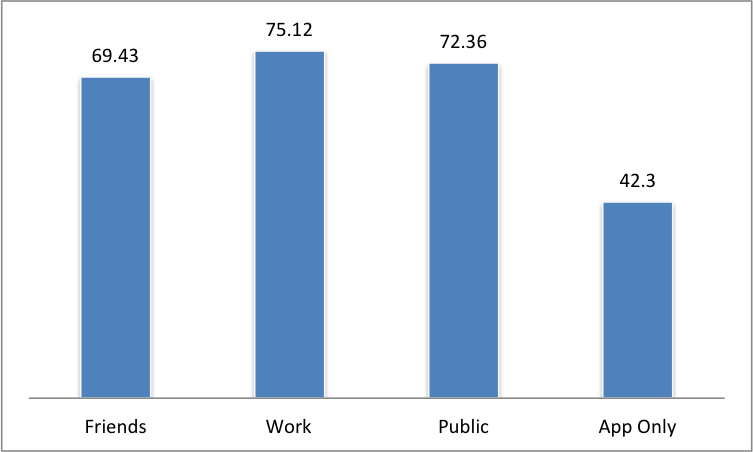
\includegraphics[width=0.5\textwidth]{recipient.png}
	\caption{(This is a placeholder! TODO: generate a better plot for data recipient)}
\end{figure}

%\begin{table}%[h]
%\begin{center}
%\begin{tabular}{llllll}
%Recipients	& Chi^2 &	2-tail P & 	Sig?	& n & Effect Size \\
%Work-App	& 564.318 & <0.0001 & Yes	& 5085 & 0.111\\
%Public-App	& 479.980 & <0.0001 & Yes	& 5192 & 0.092\\
%Friends-App & 380.000 & <0.0001 & Yes & 5098 & 0.075\\
%Friends-Work & 20.365 & <0.0001 & Yes & 5039 & 0.004\\
%Friends-Public & 5.349 & 0.0207 & No	& 5146 & 0.001\\
%Work-Public&  5.054 & 0.0246 & No & 5133	& 0.001\\
%\end{tabular}
%\caption{Results of a Chi-Squared test of the effects of various recipients contributing to VUR.}
%\label{recipient}
%\end{center}
%\end{table}

\begin{table}%[h]
\begin{center}
\begin{tabular}{| c | c | c | c |}
Recipients	& Chi^2 &	2-tail P &  Effect Size \\
Work-App	& 564.318 & <0.0001 & 0.111\\
Public-App	& 479.980 & <0.0001 &  0.092\\
Friends-App & 380.000 & <0.0001 & 0.075\\
Friends-Work & 20.365 & <0.0001 &  0.004\\
Friends-Public & 5.349 & 0.0207 &  0.001\\
Work-Public&  5.054 & 0.0246 &  0.001\\
\end{tabular}
\caption{Chi-Squared test results of the effects of various recipients contributing to VUR.}
\label{recipient}
\end{center}
\end{table}				
						
%Friends-Work	0.867	0.3517	No		604		0.001\\
%Friends-Public	1.460	0.2229	No		639		0.002\\
%Friends-App	32.066	<0.0001	Yes		609		0.053\\
%Work-Public	0.670	0.7956	No		631		0.001\\
%Work-App	42.492	<0.0001	Yes		601		0.071\\
%Public-App	48.520	<0.0001	Yes		636		0.076\\

We performed an exploratory analysis to examine the effect of data recipient using a chi square test; in order to do this, the assumption about independence of observations was violated. However, we do not believe that this impacted the outcome of the statistical test based on the randomization of treatments across all conditions, as well as the very large sample size. To examine whether the violation of this assumption impacted our results, we further created a mixed effects model, in order to isolate the subjects variable (i.e., to examine the extent to which random effects stemming from individual differences may be responsible for the effects that we observed). When we perform the same tests on many subsets of questions, with one answer randomly sampled from each participant (preserving assumption about the independence of observations), the results are still equivalent. 

\begin{table}%[h]
\begin{center}
\begin{tabular}{| l | c |}
<data> & VUR  \\
social security number & 98.04\% \\
a video of you unclothed & 97.44\% \\
bank account information & 97.10\% \\
recordings of your work conversations & 96.97\% \\
an incriminating/embarrassing photo of you & 96.36\% \\
a photo of you unclothed & 96.30\% \\
credit card information & 95.92\% \\
username and password for websites & 95.41\% \\
a video of you entering in your PIN & 93.91\% \\
recordings of your phone conversations & 93.88\% \\
\end{tabular}
\caption{A table of the top 10 upsetting <data> types, with respect to <recipient> types friends, work, and public.}
\label{sharedtop10}
\end{center}
\end{table}

\begin{table}%[h]
\begin{center}
\begin{tabular}{| l | c |}
%starting from #63
<data> &  VUR  \\
bank account information & 90.91\% \\
a video of you unclothed & 90.62\% \\
social security number  & 88.68\% \\
video of you entering your PIN & 88.57\% \\
an incriminating/embarrassing photo of you & 78.05\% \\
a photo of you unclothed & 77.78\% \\
a video of you entering a passcode to a door & 75.00\% \\
when and how much you have sex & 73.08\% \\
an incriminating/embarrassing video of you & 71.88\% \\
a random (inward-facing) photo of you at home & 66.67\% \\
\end{tabular}
\caption{A table of the top 10 upsetting <data> types, respect to <recipient> app's server only (didn't share it with anyone else).}
\label{notsharedtop10}
\end{center}
\end{table}

\begin{table}%[h]
\begin{center}
\begin{tabular}{| l | c |}
%starting from #63
<data> &  VUR  \\
your name & 47.25\% \\
when and how much you exercise & 46.07\% \\
when you were happy or having fun & 38.10\% \\
what television shows you watch & 35.96\% \\
when you are busy or interruptible & 34.34\% \\
your heart rate & 32.28\% \\
music from your device & 31.87\% \\
your age & 29.67\% \\
the language you speak & 20.95\% \\
your gender & 16.81\% \\
\end{tabular}
\caption{A table of the bottom 10 upsetting <data> types, with respect to <recipient> types friends, work, and public.}
\label{sharedbottom10}
\end{center}
\end{table}


\begin{table}%[h]
\begin{center}
\begin{tabular}{| l | c |}
%starting from #63
<data> &  VUR  \\
when and how much you exercise & 16.67\% \\
how much you use your phone & 15.79\% \\
your age & 14.29\% \\
how much you like the people you interact with & 13.79\% \\
when, what, and how much you ate & 12.50\% \\
which television shows you watch & 11.43\% \\
your gender & 9.52\% \\
your heart rate & 9.09\% \\
eye movement patterns (for eye tracking) & 6.98\% \\
the language you speak & 2.50\% \\
\end{tabular}
\caption{A table of the bottom 10 upsetting <data> types, respect to <recipient> app's server only (didn't share it with anyone else).}
\label{notsharedbottom10}
\end{center}
\end{table}


Commonly, bank info, SSN, PIN, embarrassing photo, naked photo, naked video were considered to be highly sensitive. When people perceived that the data would be shared with the app only, the other top five concerns included the passcode to a door, how frequently one has sex, embarrassing videos, and photos at home. When people perceived that the data would be shared with a human audience, their other top concerns were work conversations, credit card information, username and password combinations for websites, and phone conversations. When data is perceived to be shared by an app, people are more concerned with issues of being spied on or tracked, whereas when data is perceived to be shared with an individual, people are concerned more with theft or reputation. 

On the other hand, exercise details, age, tv shows, gender, heart rate, and language were commonly considered to be lease concerning. When people perceived that the data would be shared with the app only, the other indifferent data included phone use, how much one liked the people around, when and what you ate, and eye patterns. When people perceived that the data would be shared with a human audience, the least concerning data included one's name, if one was having fun, music on the device, and if one was busy or interruptible. When sharing with an application, information otherwise considered personal such as phone use, opinions of people, food eaten, or eye patterns were okay to share, since these seem like useful information to improve one's device experience. However, people are not likely to share the same with people, but are more comfortable with sharing data about topics which would come up in causal conversation.

\subsection{Device Type}

(REDO) So, there is a difference between the device types, but I need to do more work to see if this is statistically significant or not. In either case, this matters the least, and device type and data recipient are more influencing factors. This is just the result of biases in people we can't quite quantify.  

\begin{figure}
	\centering
	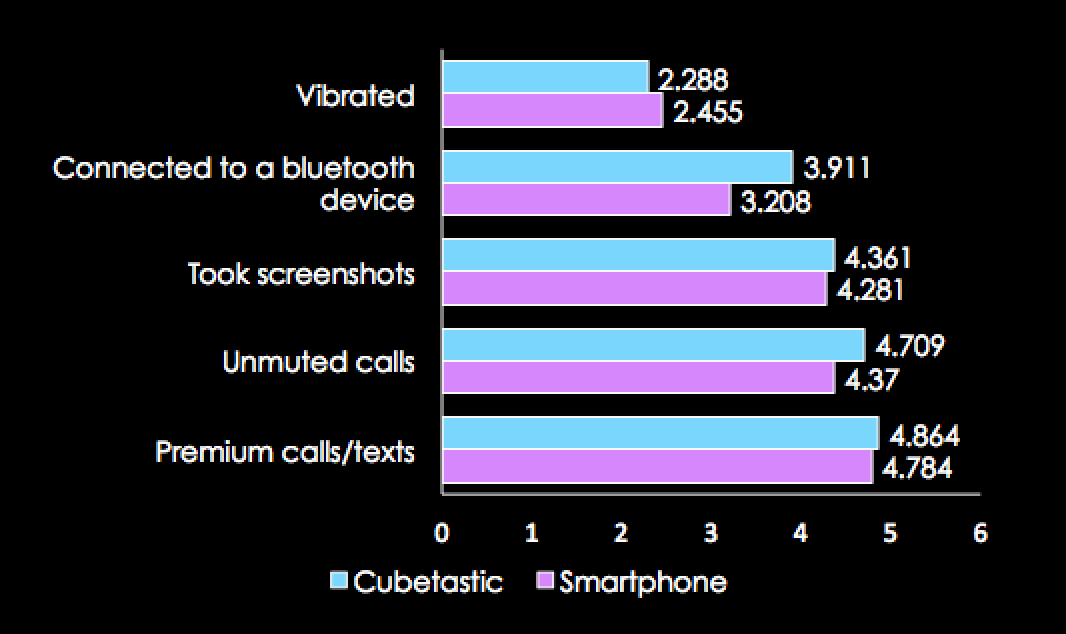
\includegraphics[width=0.5\textwidth]{device-type.png}
	\caption{(This is a placeholder! TODO: generate a better version of this)}
\end{figure}

\begin{table}%[h]
\begin{center}
\begin{tabular}{| c | c | c |}
 Question &  Wearable VUR & Smartphone VUR \\
Q1 & 14.81\%  &  6.13\%\\
Q2 & 44.11\%  &  19.85\%\\
Q3 & 87.09\%  &  58.44\%\\
Q4 & 52.77\%  & 55.79\%\\
Q5 & 86.49\%  &  91.82\%\\ 
\end{tabular}
\caption{A table of the bottom 10 upsetting <data> types, respect to <recipient> app's server only (didn't share it with anyone else).}
\label{deviceVUR}
\end{center}
\end{table}

\begin{table}%[h]
\begin{center}
\begin{tabular}{| c | c | c | c |}
%Question & Chi^2 &	2-tail P &	Sig?	 & n	& effect size\\
%All	2.814	0.1395	No		3589		0.001\\
%Q1	2.500	0.1139	No		714		0.004\\
%Q2	17.333	<0.0001	Yes		708		0.024\\
%Q3	0.020	0.8886	No		699		0.000\\
%Q4	1.426	0.2324	No		731		0.002\\
%Q5	1.611		0.2043	No		710		0.002\\
Question & Chi^2 &	2-tail P & Effect Size\\
All & 2.814 & 0.1395 & 0.001\\
Q1 & 2.500 & 0.1139 & 0.004\\
Q2 & 17.333 & <0.0001 & 0.024\\
Q3 & 0.020 & 0.8886 & 0.000\\
Q4 & 1.426 & 0.2324 & 0.002\\
Q5 & 1.611 & 0.2043 & 0.002\\
\end{tabular}
\caption{Results of the effects of <device> type contributing to VUR. Values are Chi-Square test results for between-subjects comparisons for participants who received one question, but not the other.}
\label{betweendevice}
\end{center}
\end{table}
						
\begin{table}%[h]
\begin{center}
\begin{tabular}{| c | c | c | c |}
%Question & Chi^2 &	2-tail P & Sig? & Odds ratio	 & Confidence& Odds range\\
%All		0.444	0.505	No	0.5		95\%			0.081 to 2.341\\
%Q1		0		1		No	n/a	         n/a	                  n/a\\
%Q2		0		1		No	0.5		95\%	                  0.008 to9.605\\
%Q3		0		1		No	n/a	         n/a	                  n/a\\
%Q4		0		1		No	0.5		95\%			0.008 to9.605\\
%Q5		0		1		No	n/a	         n/a	                  n/a\\
Question & Chi^2 &	2-tail P & Effect Size \\
All & 0.444  & 0.505 & 0.006\\
Q1 & 0 & 1 & 0 \\
Q2 & 0 & 1 & 0\\
Q3 & 0 & 1 & 0\\
Q4 & 0 & 1 & 0\\
Q5 & 0 & 1 & 0\\
\end{tabular}
\caption{Results of the effects of <device> type contributing to VUR. Values are McNeamar's test results for within-subjects comparisons for participants who received both questions.}
\label{withindevice}
\end{center}
\end{table}

For the between-subjects comparison (i.e., participants who received one question, but not the other), you can do either a chi-square test or Fisher's exact test. Both use a 2 x 2 contingency matrix (i.e., rows are outcomes---upset or not---and columns are conditions---wearable or smartphone). The way to choose between the two tests is based on sample size, generally you use chi-square when there are more than 10-20 samples per cell in the table, but using either is just as valid. For the within-subjects comparisons (i.e., participants received both questions), you would do McNemar's test; which is the within-subjects version of the chi-square test. 

Exact question details here, and statistical stuff. Conclude with whatever conclusion I happen to come to after performing the statistical analysis. 

\subsection{Regression Model} 
Introduce the model and what was considered in the model. Serge can probably do this better. Talk about which factors mattered, and how much, and also interesting statistics we found, if any. Also, correlations with demographics here as well! 

%I didn't do the correlation yet
(EXAMPLE) We found that the very upset rate for participants was not correlated with (pick correct ones from IUIPC, age, gender, education, wearable ownership) (give correlation coefficients), positively correlated with  (IUIPC, age, gender, education, wearable ownership) (give correlation coefficients), and negatively correlated with  (IUIPC, age, gender, education, wearable ownership) (give correlation coefficients). 

Because wearable devices have been adopted by a younger, rich, technology-savvy demographic  \cite{cmo}, it is natural to see that younger or more educated participants have had a more favorable view of wearable devices. This may be due to cultural exposure through marketing or friends, or an attitude of openness to new technologies. Participants who had a higher IUIPC score, which infers a higher sensitivity to privacy, were more likely to be upset at the various scenarios which may occur when wearing a wearable device. Additionally, these people were more likely to be adverse to these technologies for the sake of preserving privacy, whether they had explicit concerns or a vague feeling of uneasiness. There was no correlation between a person's gender and their views of wearable devices, reaffirming that wearable devices are equally exposed to both genders. 


\subsection{Risk and Benefit Ranks} 
When assessing new technologies, participants generally had rated the technologies similarly, considering them low risk and low benefit (see figure \ref{fig:techplot}). We suspect that these similar assessments are because most are not consciously aware of the possibilities of these technologies or how they are being used today. A list of the ranking of most risky and most beneficial technologies can be see in appendix \ref{sec:techrank}; the most risky and most beneficial technologies reveals the list of most familiar technologies for the average user (internet, laptops, email, smartphones, etc.). 

%should I just put the list in here, in the main part of the paper?

\begin{figure}
	\centering
	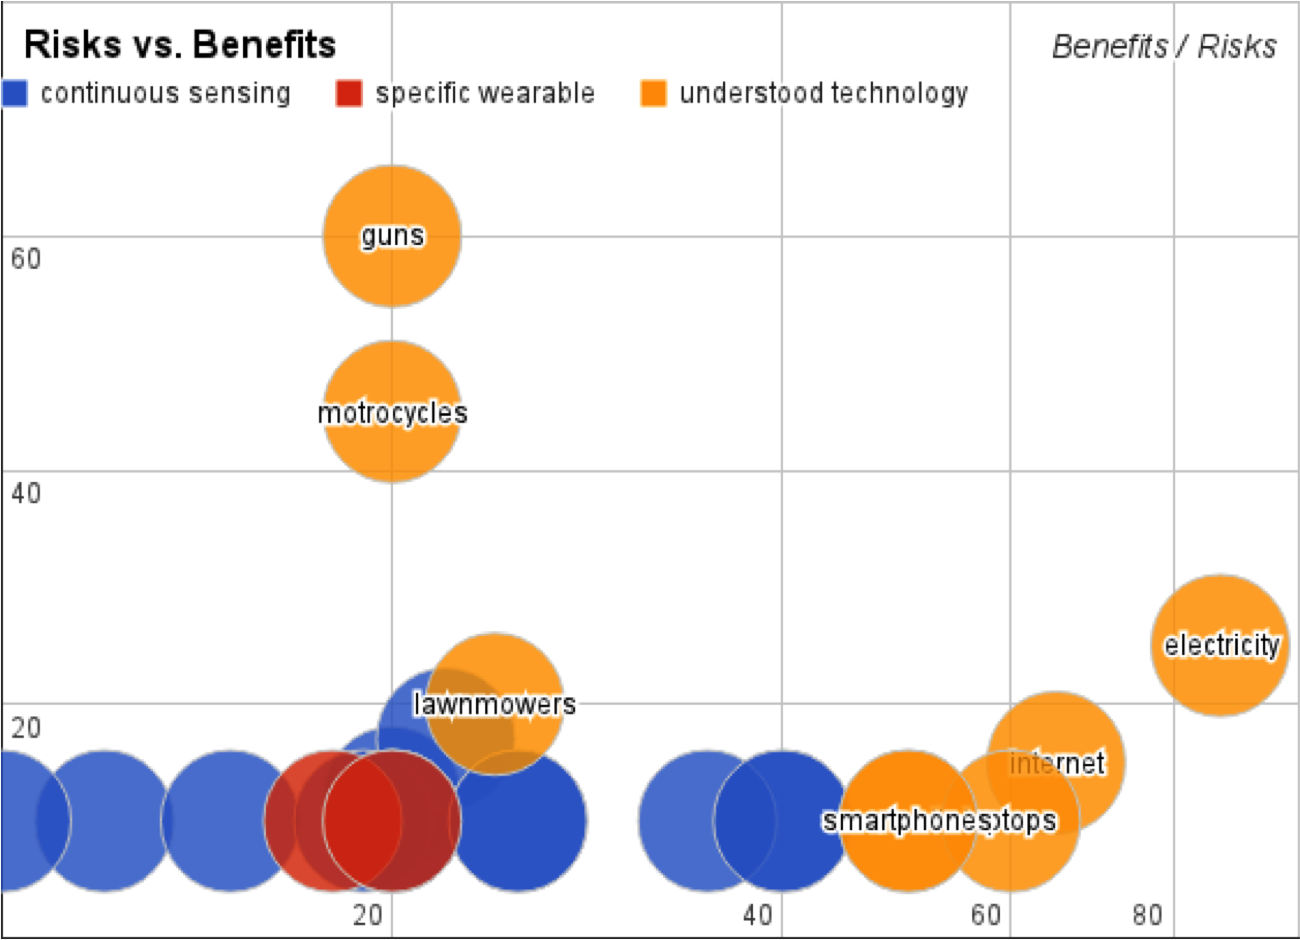
\includegraphics[width=0.5\textwidth]{techplot.png}
	\caption{(This is a placeholder! TODO: generate a better plot; take out the specific wearables too.)}
	\label{fig:techplot}
\end{figure}

Notably, technologies perceived to be beneficial include location tracking and heart rate detection. Again, we believe this is the result of exposure people have to these technologies--most people use GPS or other location-based applications on their smart phones and fitness trackers are the most popular type of wearable device. Technologies considered to be risky, such as a discrete camera and facial detection, seemed to be based on media exposure or general aversion to privacy invasion. However, people are becoming increasingly aware of such risks and are comparing these risks of privacy invasion to real physical risks--for instance, the capacity for facial detection on a wearable device is perceived to be almost as risky as interacting with a physical lawnmower. It is fair to say that, these assessments of the most risky or beneficial technologies may not be the most accurate, but do reflect the exposure of various technologies to the general public and also prove that people do perceive risks in a real way related to these technologies. 

\subsection{Perceived Concerns for Wearable Devices}
So far, participants had responded to questions regarding specific scenarios or assessed technologies presented to them. For completeness of the survey, we also wanted to capture the participants' general reactions to wearable devices as a whole. To do this, we asked the participants an open-ended question regarding the most likely risks associated with owning and interacting with wearable devices.

\textit{What do you think are the most likely risks associated with wearable devices?}\\[-.5cm]

This question was asked along with the demographics questions, near the end of the survey, but before any IUIPC questions regarding privacy, to avoid biasing. The participants were presented with a blank box to write in, with no character limit to their open-ended responses. 

Without any doubt, the open-ended responses state that the most common concern for owning and interacting with wearable devices for the average user is the \textit{possible loss of privacy}. This top concern surpassed all other concerns by about an order of magnitude or more:

\begin{table}[h]
\begin{center}
\begin{tabular}{lll}

Concern &  Responses &  Frequency &   \\
Privacy & 452 & 25.32\% \\
Being Unaware & 275 & 15.40\ \\
%Unaware Use & 167 & (9.36\%)\\
%Unaware Collection & 64 & (3.59\%)\\
%Unaware Access & 44 & (2.46\%)\\
Health Risk & 191 & 10.70\%\\
Safety & 186 & 10.42\%\\
Financial Cost & 151 & 8.46\%\\
Security &	144 & 8.07\%\\
Social Impact &	157 & 8.80\%\\
Accidental Sharing &	69 & 3.87\%\\
Miscellaneous &	57 & 3.19\%\\
None	& 51 & 2.86\%\\
Social Stigma &	39 & 2.18\%\\
False Information & 33 & 1.85\%\\
Don't know & 31 & 1.74\%\\
Aesthetics 	& 19 & 1.06\%\\
Don't care 	& 11 & 0.62\%\\

\end{tabular}
\caption{A table listing the self-reported most common risks associated with owning a wearable device.}
\label{open-responses}
\end{center}
\end{table}

Other significant secondary concerns included being unaware of what the device is collecting, doing, or which information it is using (Being Unaware), long-term health effects caused from wearing the device such as cancer from emf waves (Health), safety hazards from wearing the device such as battery burns or distractions causing car accidents (Safety), the high financial cost of buying, replacing, or caring for the device (Financial),  information compromise (Security), and resulting changes in social behaviors, such as dependencies on devices or spending less time with loved ones (Social Impact). Refer people to the appendix \ref{sec:coding} for detailed information on coding labels. 

%%%%%%%%%%%%%%%%%%%

\section{Discussion}
We take this section to discuss complementary future research directions in fields of privacy, ubiquitous computing, and user studies, along with specific limitations of this survey. 

\subsection{Future Research Directions}
(REDO, ask David's/Serge's input for this section) Additional future work is encouraged in the area of studying privacy with respect to ubiquitous computing, since we proved it was the number one concern of the users of wearable devices. Clearly, this is a hard question which has been worked on for a long time but not yet fully addressed. Even this survey just barely touched on the various factors which can influence privacy perceptions and how upset people would be. 

 Also, maybe some work with respect to security threats, and how feasible they might be, and some defenses against stopping wearables devices from getting sensitive information (like blocking text, detecting sensitive situations like the bathroom, etc.). Research which defends against false information, false positive commands, and just more safeguards against the new system for wearables, whatever that is, is also something to really look into. 
 
 Work making sure that people are aware of what is going on, using indicators, not-too-transparent interfaces, and maybe being polite (recording rules follow social rules--think polite glass talk from Jaeyeon at MSR) are going to be valuable as wearables get more sophisticated but also more adopted by people. Think about it--put people in control of the technology, not technology shifting the social norms (our survey says that one of the top concerns of people were about how wearables will change social norms). 

\subsection{Limitations}
One of the main limitations of this work is that our participants might not have interest, or an accurate idea, of wearable devices and their capabilities. 83\% of our participants reported that they do not own a wearable device, but at this time, about ~15\% of the general population own and use wearable devices \cite{Nilsen}\cite{WearableStatNews}, so our study is reflective of the status quo. We believed that getting a representative survey base was a useful endeavor, although we could have easily recruited only wearable device owners or people specifically interested in wearables. However, that will also have its own bias and limitations as well, since they would not reflect the general population. We expect user perceptions to change as rapidly as wearable technologies and the rate of adoption change. 

Crowdourcing user studies in Mechanical Turk has its challenges \cite{kittur2008crowdsourcing}. While the Amazon Mechanical Turk population is diverse across several significant demographic dimensions such as age, gender, and income, it is not a precise representation of the U.S. population \cite{ross2010crowdworkers}\cite{kelley2010conducting}. Additionally, Amazon Mechanical Turk workers generally put a higher value on anonymity and hiding information, were more likely to do so, had more privacy concerns than the larger U.S. public \cite{kang2014privacy}. 

The survey was constructed in a way to randomize the order of the particular sets of questions participants saw, except for the open-ended question, which was always near the end of the survey, asked along with the demographics. For this reason, people were heavily primed for the open-ended question. However, this question was always shown before the IUIPC questions, so our results on privacy being the top concern isn't because of the bias from the privacy index. The intent of the open-ended question  was more to get a sense of what people were concerned of, and we believe the results do reflect their actual concerns, but with a bit more clarity, since the participants were already thinking about such risks related to wearables. 

(REDO, Should I even say this?) I messed up that motorcycle question. I wish I actually had a calibration point for high risk high benefit for the Fischoff technology assessment questions. But well, none of the new technologies fit that description so we didn't really need it critically. 

%%%%%%%%%%%%%%%%%%%

\section{Conclusion}
(REDO) END STRONG! Should I put this before the Discussion?  Echo the introduction a little, remind the people of the takeaways in a way that highlights the contribution of this paper. Intro: ``we studied user perceptions for threats in wearable devices, along with user perceptions of risk and benefit for emerging technologies and what they thought was the biggest risk for using wearable devices. Data type, data recipient, and device type all matter different amounts. All new technologies were perceived to be low risk low benefit but we think this is because people are unfamiliar with these technologies. Privacy was the number one concern, followed by security, then health, money, social norms changing and social stigma. Fantastic ending sentence here.''

I can talk about the results a little bit more in depth because people have already supposedly read my whole paper now. Pull out the subtleties I couldn't have done in the introduction, and go into specific details, shooting out numbers and statistics. Then conclude the whole thing with an inspirational pitch on how there is much future work to be done in this area, how this area is exciting, and how I basically helped people see both of these things. 

%\end{document}  % This is where a 'short' article might terminate

%ACKNOWLEDGMENTS are optional
\section{Acknowledgments}
NSF funding, SCRUB, BLUES. Also any people who helped.


%%%%%%%%%%%%%%%%%%%
%%%            BIB & ACKS          %%%
%%%%%%%%%%%%%%%%%%%

% The following two commands are all you need in the initial runs of your .tex file to produce the bib
%  and remember to run: latex bibtex latex latex to resolve all references

\bibliographystyle{abbrv}
\bibliography{wearables_survey}  % wearables_survey.bib is the name of the Bibliography


%APPENDICES are optional
%\balancecolumns
\appendix
%Appendix A
\section{Fischoff Prompts}
\label{sec:prompt}

BENEFIT prompt: 


``We would like to ask you to rate the benefits associated with each of the following technologies.  \\[-.6cm]

Consider all types of benefits: how many jobs are created, how much money is generated directly or indirectly, how much enjoyment is brought to people, how much a contribution is made to the people's health and welfare, what this technology promotes, and so on. (e.g. for swimming, consider the manufacture and sale of swimsuits, the time spent exercising, the social interactions during swimming, and the sport created around the activity.) Give a global estimate over a long period of time (say, a year) of both intangible and tangible benefits. \\[-.6cm]

Do not consider the costs or risks associated with these items. It is true, for example, that sometimes swimmers can drown. But evaluating such risks is not your present job. Your job is to assess the gross benefits, not the net benefits which remain after the costs and risks are subtracted out. \\[-.6cm]

Please rate the following technologies below with a number. We know that this might be a bit hard to do, but please try to be as accurate as possible, adjusting the numbers until they feel they are right for you. Start with the least beneficial technology at 10 and assign higher numbers for the more beneficial technologies. (For instance, a technology rated 34 is twice as beneficial as a technology rated 17)''

RISK prompt:

``We would like to ask you to rate the risks associated with each of the following technologies. \\[-.6cm]

Consider all types of risks: the risk of physical harm or death, the risk to others or bystanders, the financial cost of the technology, any distress caused by the technology, what the consequences would be if the technology was misused, any impact on the public, work, or personal life, and other considerations. (e.g. for electricity, consider the risk of electrocution, the pollution caused by coal, the risk that miners need to take to mine the coal, the cost to build the infrastructure to deliver electricity, etc.) Give a global estimate over a long period of time (say, a year) of both intangible and tangible risks. \\[-.6cm]

Do not consider the costs or benefits associated with these items. It is true, for example, that electricity also creates a market for home appliances. But evaluating such benefits is not your present job. Your job is to assess the gross risks, not the net risks which remain after the costs and risks are subtracted out.\\[-.6cm]

Please rate the following technologies below with a number. We know that this might be a bit hard to do, but please try to be as accurate as possible, adjusting the numbers until they feel they are right for you. Start with the least risky technology at 10 and assign higher numbers for the more risky technologies. (For instance, a technology rated 14 is half as risky as a technology rated 28.)''

\section{Risk and Benefit Rankings}
\label{sec:techrank}

BENEFIT: 

technology 	median	25\%		75\% \\
electricity	87	50	100\\
internet	65	45	100\\
laptops	60	40	80\\
email	50	30	75\\
smartphones	50	32.5	75\\
location tracking	40	20	67.5\\
heart rate detection	40	28	62.5\\
language detection	35	15	60\\
voice recognition	25	15	40\\
speech to text	25	15	36.25\\
lawnmowers	24	15	40\\
facial recognition	22	13	40\\
guns	20	10	30\\
motrocycles	20	12	40\\
voice based emotion detection	20	10	30\\
facial detection	20	10	32\\
discrete camera	20	15	30\\
smartwatches	20	10	32.5\\
google glass	20	12	40\\
fitness trackers	19	10	30\\
cubetastic	18	10	30\\
discrete microphone	15	10	20\\
age detection	12	10	21\\
gender detection	10	10	15

RISK: 

technology 	median	25\%		75\%\\
guns	60	40	80\\
motrocycles	45	27	70\\
electricity	25	15	40\\
lawnmowers	20	12	30\\
facial recognition	17	12.5	30\\
internet	15	10	30\\
discrete camera	12	10	30\\
location tracking	10	10	20\\
age detection	10	10	15\\
gender detection	10	10	12\\
language detection	10	10	10\\
voice based emotion detection	10	10	15\\
facial detection	10	10	25\\
voice recognition	10	10	15\\
heart rate detection	10	10	10\\
email	10	10	16\\
speech to text	10	10	10\\
discrete microphone	10	10	20\\
smartphones	10	10	19\\
laptops	10	10	15\\
fitness trackers	10	10	10\\
smartwatches	10	10	10\\
google glass	10	10	20\\
cubetastic	10	10	30

\section{Coding Label Definitions}
\label{sec:coding}

Privacy: ``privacy,'' revealing personal information, spying. \\
Security:  ``security,'' compromise, malware, hacking. \\
GPS tracking: ``location,'' ``GPS,'' being monitored. 

Unaware use: using data without permission or in a different way than understood by user. \\
Unaware collection: collecting data without permission. \\
Unaware access: disclosure of data without permission. \\
False information: inaccurate or maliciously false data.

Health Risk: radiation, cancer, or long-term effects.\\
Safety: distractions causing car crashes or injuries, mugging or violence because of the device, injuries from device malfunctions (battery burns).\\
Discomfort: eye strain, headache, obscured vision, irritation. \\
Financial cost: getting ripped off by buying the device or device accessories, having to buy another device when broken or stolen, financial compromise caused by device. \\
Theft: the device getting stolen. 

Social Impact: dependency, distance from friends and family, changes in decision making, social changes, etc. \\
Social Stigma: judgment, hate, or bystander discomfort.\\ 
Aesthetics: fashion, the device being ugly, mentions of not looking cool/dorky. 

Miscellaneous: odd comments, uncommon concerns. \\
None: ``None,'' no threat, perceiving no big concerns \\
Don't know: ``do not know,'' hinting at confusion \\
Don't care: `` do not care,'' nonchalant answers 


%\section{Detailed Tech Rankings}

\balancecolumns

% That's all folks!
\end{document}
\\